\chapter{插入图片}
示例内容

\section{二级标题}
示例内容
\subsection{三级标题}

插入图片:显著性的样例图片,固定长度
\insertfixpic{../figures/fig_sal_res1.png}{一个显著性的例子}{fig:fig1}
插入图片,自定义大小
\insertpic{1.0cm}{../figures/stop.jpg}{另一个自定义大小的例子}{figref:hahaha}


这样可以指向上面的图片与公式,如图\myref{figref:hahaha}与式\myref{equ:saliency},点击试试。


图\myref{fig:example}是显著性对象的5个例子,图\myref{example_sub3_sal}是一个五角星。

\begin{figure}[htbp]
\centering  %图片全局居中
\subfigure[示例1]{
\label{example_sub1}
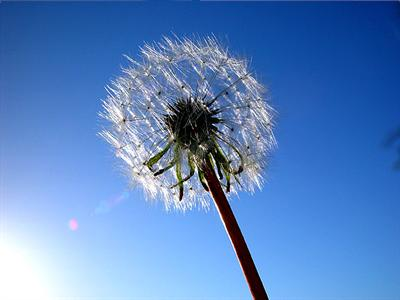
\includegraphics[width=2.7cm,height=1.8cm]{../figures/ex1.jpg}
}
\subfigure[示例2]{
\label{example_sub2}
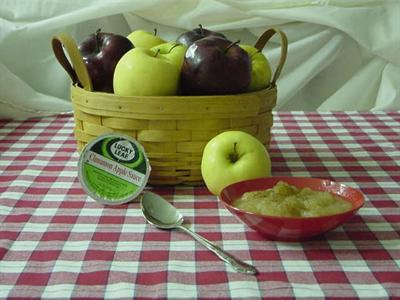
\includegraphics[width=2.7cm,height=1.8cm]{../figures/ex2.jpg}
}
\subfigure[示例3]{
\label{example_sub3}
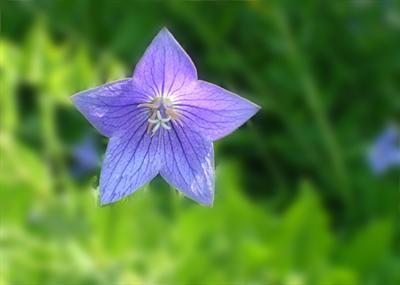
\includegraphics[width=2.7cm,height=1.8cm]{../figures/ex3.jpg}
}
\subfigure[示例4]{
\label{example_sub4}
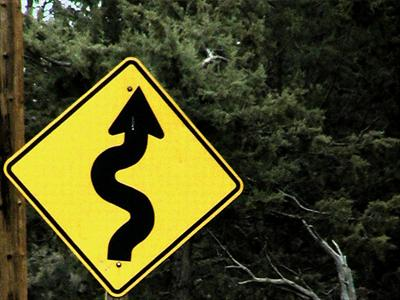
\includegraphics[width=2.7cm,height=1.8cm]{../figures/ex4.jpg}
}
\subfigure[示例5]{
\label{example_sub5}
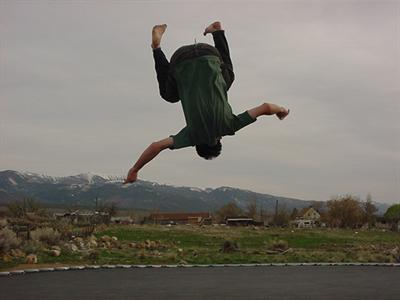
\includegraphics[width=2.7cm,height=1.8cm]{../figures/ex5.jpg}
}
\subfigure[示例1-显著对象]{
\label{example_sub1_sal}
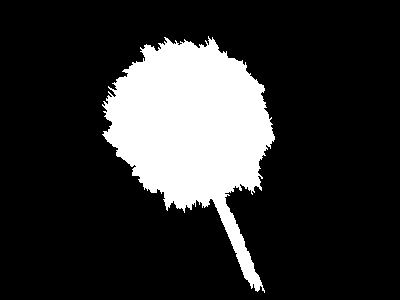
\includegraphics[width=2.7cm,height=1.8cm]{../figures/ex1.png}
}
\subfigure[示例2-显著对象]{
\label{example_sub2_sal}

\includegraphics[width=2.7cm,height=1.8cm]{../figures/ex2.png}
}
\subfigure[示例3-显著对象]{
\label{example_sub3_sal}

\includegraphics[width=2.7cm,height=1.8cm]{../figures/ex3.png}
}
\subfigure[示例4-显著对象]{
\label{example_sub4_sal}

\includegraphics[width=2.7cm,height=1.8cm]{../figures/ex4.png}
}
\subfigure[示例5-显著对象]{
\label{example_sub5_sal}

\includegraphics[width=2.7cm,height=1.8cm]{../figures/ex5.png}
}
\caption{\songti\zihao{5}这是显著性对象的样例}
\label{fig:example}
\end{figure}




自然神论、浪漫主义等思想的兴起使人们开始欣赏和赞美自然的野性,这种对自然态度和自然概念理解的变化,以及在工业城市社会日益兴盛的博物学需求,共同促使保护“自然面貌”原则在19世纪英国的形成。16、17世纪欧洲的天文学、物理学开始突破中世纪神学的思想禁锢,揭示出广袤复杂宇宙所具有的和谐面,由此科学家们更加坚信世界的“神圣来源”。这种不断增加的关于太阳系的知识逐步延伸到自然地貌当中。结果,将自然与上帝相联系的自然神论思想使人们对野生自然概念的理解产生了显著变化。例如,在17世纪早期,英国诗人把山形容为地球表面的“瘤子、疣、水泡、脓疮”等,英国一些山峰在当时被称为“魔鬼的屁股”(Devils-Arse)。但到了该世纪末期,一种相反的态度出现了。托马斯·伯内特(Thomas Burnet,1635-1715年)的《地球的神圣理论》(Sacred Theory of the Earth,1681年)、约翰·雷(John Ray,1627-1705年)的《造物中展现的神的智慧》(Wisdom of God Manifested in the Works of the Creation,1691年)②等著述运用神学和地理学的论据提出了一种可能性——山也是上帝的手泽。这种把自然神圣化的观念使人们对野生自然亦具有“美”的特质的认识逐步加深。



图片下的序号与名字在学校的要求里面是宋体小四,在学校的例子里是黑体小四。


呵,学校。


\subsection{三级标题}
示例内容



\begin{table}[htbp]
  \centering
  \caption{\songti\zihao{5}自适应阈值-减小步长寻找更优阈值}
  \label{table:adaptive_parameters_more}
  \setlength{\tabcolsep}{5mm}{
  \begin{tabular}{ccccc}
    \toprule
    倍数 & 平均精确率 & 平均召回率 & F-score & 计算耗时 \\
    \midrule
    1.25  &  81.4937\%  &  67.8341\%   & 74.0392\% & 23s \\
    1.30  &  80.2888\%  &  68.7326\%  &  74.0627\% & 22s \\
    1.35  &  79.2812\%  &  69.7478\%   & 74.2096\% & 23s \\
    1.40  &  78.0842\%  &  70.5439\%  &  74.1228\% & 22s \\
    1.45  &  77.0670\%  &  71.4551\%   & 74.1550\% & 22s \\
    1.50  &  75.9396\%  &  72.3223\%   & 74.0869\% & 22s \\
    1.55  &  74.5063\%  &  73.0072\%   & 73.7492\% & 21s \\
    1.60  &  73.2367\%  &  73.8578\%   & 73.5459\% & 21s \\
    1.65  &  72.0713\%  &  74.5796\%   & 73.3040\% & 21s \\
    \bottomrule
  \end{tabular}}
\end{table}
